\documentclass[tikz,border=1.35mm]{standalone}

\definecolor{fvmadaptedge}{HTML}{8A7E7E}
\usetikzlibrary{arrows.meta}

\definecolor{externalface}{HTML}{8FB9E8}
\definecolor{splitred}{HTML}{AF2525}

% Prism split code 2: split the two triangular end faces and connect their
% face centers. For a root triangular prism this creates three Prism(4)
% children, geometrically quadrilateral-prism columns.
\begin{document}
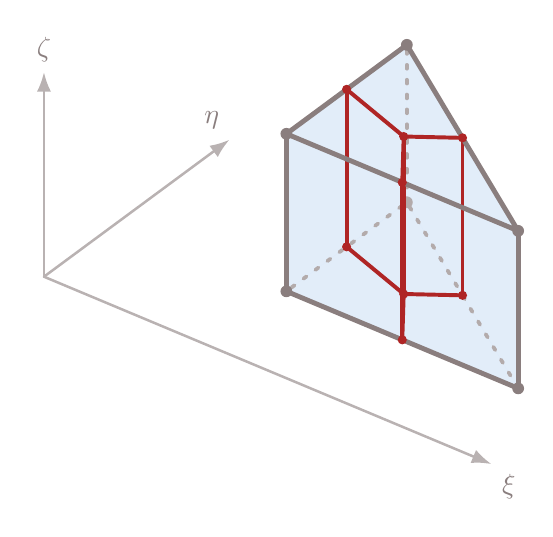
\begin{tikzpicture}[
  x={(20.3mm,-8.5mm)},
  y={(15.3mm,11.3mm)},
  z={(0mm,20mm)},
  line join=round,
  line cap=round,
  outer/.style={draw=fvmadaptedge,line width=0.62mm},
  hidden/.style={draw=fvmadaptedge!65,line width=0.48mm,loosely dotted},
  face/.style={fill=externalface,fill opacity=0.14,draw=none},
  split/.style={draw=splitred,line width=0.50mm},
  axis/.style={draw=fvmadaptedge!60,line width=0.32mm,-{Latex[length=2.5mm,width=1.8mm]}}
]
  % Right-triangular prism vertices, stretched in xi for visual clarity.
  \coordinate (A) at (0,0,0);
  \coordinate (B) at (1.45,0,0);
  \coordinate (C) at (0,1,0);
  \coordinate (D) at (0,0,1);
  \coordinate (E) at (1.45,0,1);
  \coordinate (F) at (0,1,1);

  % End-face edge midpoints and face centers.
  \coordinate (mAB) at (0.725,0,0);
  \coordinate (mBC) at (0.725,0.5,0);
  \coordinate (mCA) at (0,0.5,0);
  \coordinate (mDE) at (0.725,0,1);
  \coordinate (mEF) at (0.725,0.5,1);
  \coordinate (mFD) at (0,0.5,1);
  \coordinate (fABC) at (0.483,0.333,0);
  \coordinate (fDEF) at (0.483,0.333,1);

  % Offset computational-coordinate axes.
  \coordinate (Oaxis) at (-1.20,-0.42,-0.18);
  \draw[axis] (Oaxis) -- (1.60,-0.42,-0.18) node[below right,font=\normalsize,text=fvmadaptedge] {$\xi$};
  \draw[axis] (Oaxis) -- (-1.20,1.12,-0.18) node[above left,font=\normalsize,text=fvmadaptedge] {$\eta$};
  \draw[axis] (Oaxis) -- (-1.20,-0.42,1.12) node[above,font=\normalsize,text=fvmadaptedge] {$\zeta$};

  % Faint exterior faces keep the parent prism readable.
  \path[face] (A) -- (B) -- (C) -- cycle;
  \path[face] (D) -- (E) -- (F) -- cycle;
  \path[face] (A) -- (B) -- (E) -- (D) -- cycle;
  \path[face] (B) -- (C) -- (F) -- (E) -- cycle;
  \path[face] (C) -- (A) -- (D) -- (F) -- cycle;

  % Hidden parent geometry.
  \draw[hidden] (B) -- (C) -- (A);
  \draw[hidden] (C) -- (F);
  \fill[fvmadaptedge!65] (C) circle[radius=0.75mm];

  % End-face split scaffolds.
  \foreach \p in {mAB,mBC,mCA} {
    \draw[split] (fABC) -- (\p);
  }
  \foreach \p in {mDE,mEF,mFD} {
    \draw[split] (fDEF) -- (\p);
  }

  % Side-face split lines and the internal edge between end-face centers.
  \draw[split] (mAB) -- (mDE);
  \draw[split] (mBC) -- (mEF);
  \draw[split] (mCA) -- (mFD);
  \draw[split] (fABC) -- (fDEF);

  % Visible exterior wireframe.
  \draw[outer] (A) -- (B);
  \draw[outer] (D) -- (E) -- (F) -- cycle;
  \draw[outer] (A) -- (D);
  \draw[outer] (B) -- (E);

  % Original vertices are #8a7e7e.
  \foreach \p in {A,B,D,E,F} {
    \fill[fvmadaptedge] (\p) circle[radius=0.75mm];
  }

  % Edge and face refinement nodes are red.
  \foreach \p in {mAB,mBC,mCA,mDE,mEF,mFD,fABC,fDEF} {
    \fill[splitred] (\p) circle[radius=0.58mm];
  }
\end{tikzpicture}
\end{document}
